\section{Statistiche Repository}
\subsection{Premessa}\label{PremessaStats}
Per trasparenza e concretezza dei dati riportati questi fanno riferimento ai periodi di attività del team, non saranno quindi considerati nei calcoli il periodo compreso tra il 19 Ottobre e il 15 Novembre e la settimana del 28 Settembre, nella quale è stato creato il repository, ma che non ha visto ulteriori svolgimenti. Inoltre è bene notare che il primo dei due periodi di attività fa riferimento esclusivamente all'inizio dell'analisi della consegna e della stesura delle documentazione con Glossario\sref{Glossario}, Analisi dei Requisiti\sref{RequisitiNonFunzionali}\textsuperscript{,}\sref{RequisitiDominio}, Scrittura degli use case diagrams\sref{UseCaseDiagrams}, Formalizzazione dei casi d'uso\sref{FormalizzazioneUseCase} e creazione di Personas\sref{Personas}; quindi durante questa prima fase non sono stati prodotti artefatti software. I dati sono aggiornati al giorno 26/12/2025 

\subsection{Analisi dei Contributors}
\begin{figure}[H]
        \centering
        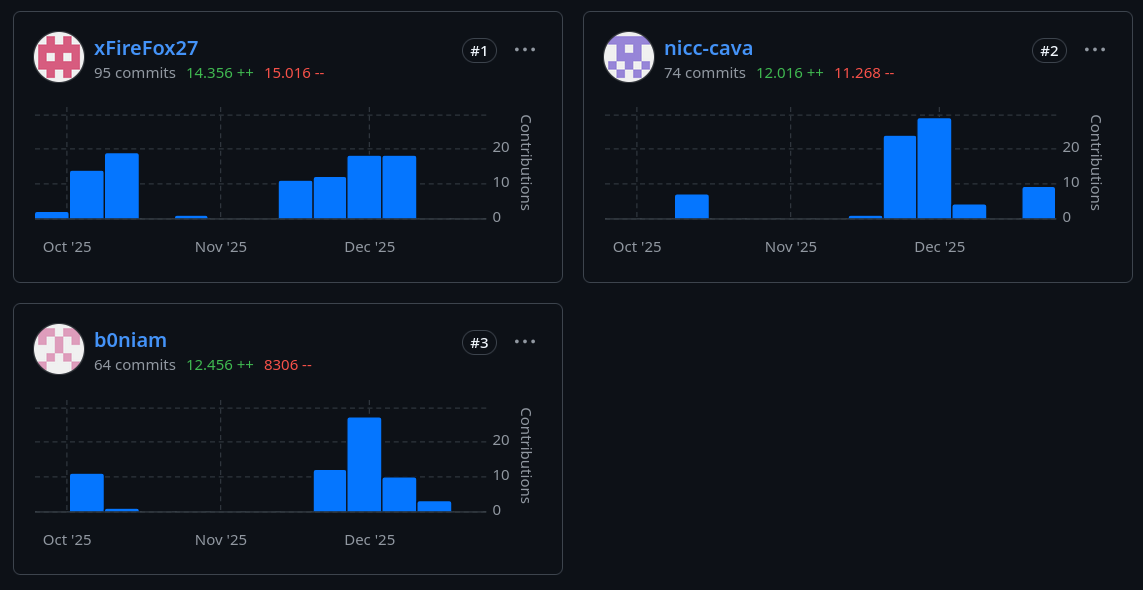
\includegraphics[width=1\linewidth]{src/statistiche-repository/Contributors.png}
        \caption{Screenshoot dei Contributors, da GitHub}\label{ScreenshootContributors}
\end{figure}
Come evincibile dalla schermata dei contributors\sref{ScreenshootContributors} il lavoro è stato diviso piuttosto equamente con una media di circa 76 commit a contributore, 12.189 linee di codice inserite e 11.326 linee di codice eliminate.

\subsection{Analisi dei Commit}
\begin{figure}[H]
        \centering
        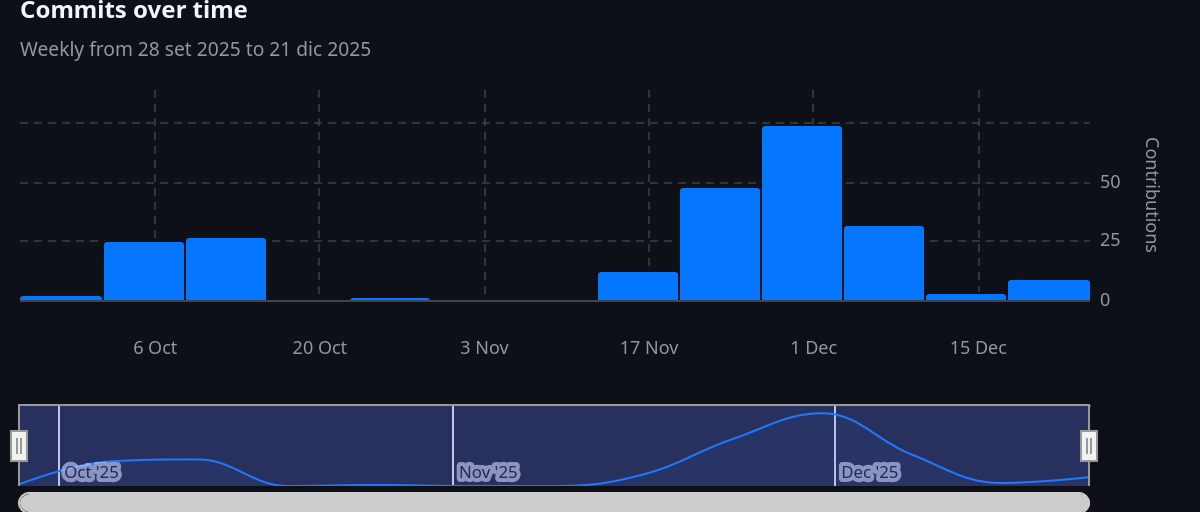
\includegraphics[width=1\linewidth]{src/statistiche-repository/Commits over time.png}
        \caption{Screenshoot dei Commits over time, da GitHub}\label{ScreenshootCommits}
\end{figure}
Il repository, nei periodi di attività sopra indicati\sref{PremessaStats}, ha visto 232 commits con una media di 29 commits a settimana durante i due distinti periodi. Facendo riferimento ai singoli periodi, invece, abbiamo un totale di 52 commit e una media settimanale di 26 commit per il primo e 180 totali con una media di 30 commit a settimana per il secondo.

\subsection{Analisi delle Linee di Codice}
\begin{figure}[H]
        \centering
        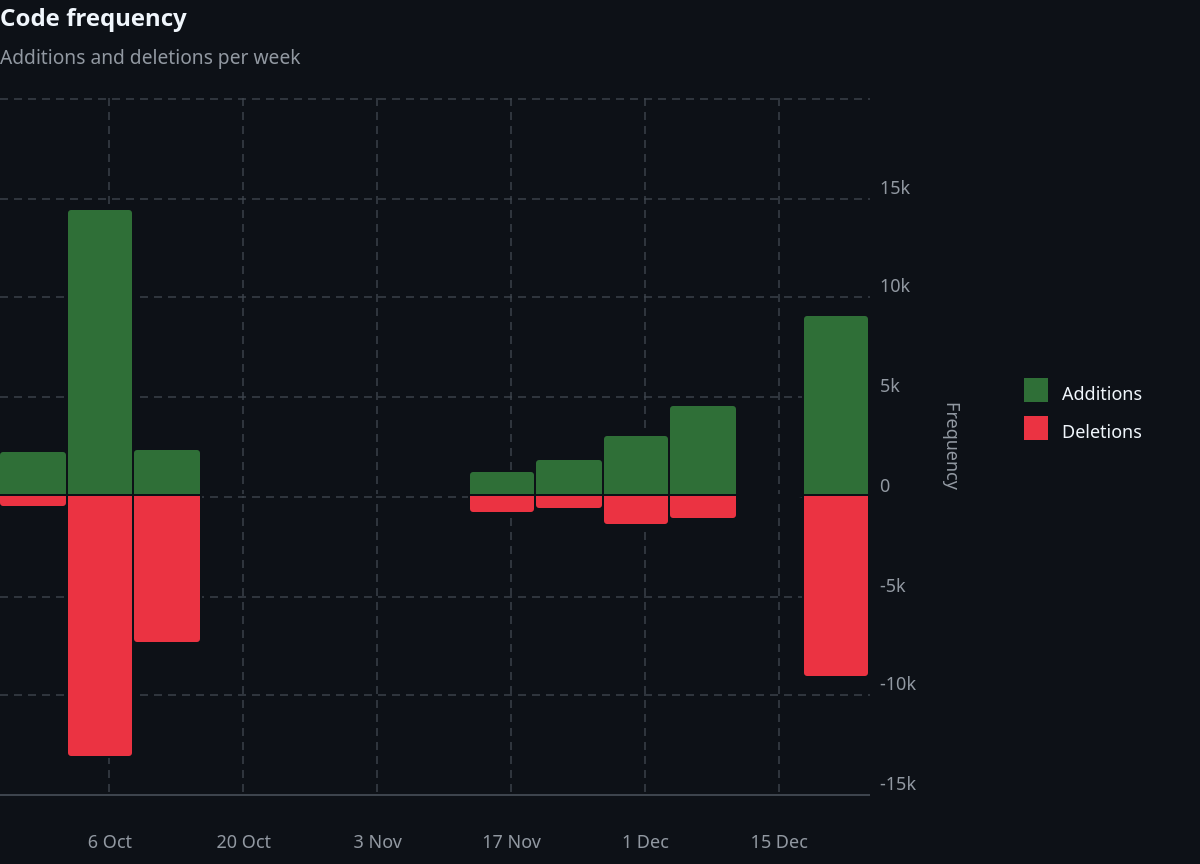
\includegraphics[width=1\linewidth]{src/statistiche-repository/Code frequency.png}
        \caption{Screenshoot della "Code Frequency", da GitHub}\label{ScreenshootCodeFrequency}
\end{figure}
Facendo riferimento ai periodi di attività sopra citati\sref{PremessaStats}, il repository ha visto l'inserimento di 36.569 linee di codice con una media di 4.571 a settimana, delle quali 16.739 con circa 8.370 di media settimanale sono state inserite nel primo dei due periodi mentre 19.830 inserimenti totali con media settimanale di 3.305 nel secondo, e la rimozione di 33.978 con una media di 4.247 rimozioni per settimana divise in 20.554 nel primo periodo con una media di 10.277 settimanale e le restanti 13.424 nel secondo con una media settimanale di 2.237 rimozioni.